Considerando, ora, la stessa architettura software precedentemente utilizzata, si potrebbe mettere il luce un possibile problema: impiego di risorse aggiuntive a causa di istruzioni logiche condizionali. In particolare, questo problema è dovuto al fatto che, all'interno del ciclo for, è prevista l'istruzione condizionale $if(i == 0)$ che comporta l'utilizzo di risorse hardware addizionali. Bisogna precisare che, istruzioni logiche quali $if$, $else$ e $then$ rendono i loop inefficienti limitando le performance dal punto di vista hardware.
Fondamentalmente, l'istruzione condizionale $if(i == 0)$ a livello hardware si traduce nel leggere il valore dell'indice $i$ in una certa struttura dati ed effettuare il confronto, tramite un comparatore, tra tale valore appena citato e il valore zero.

\lstinputlisting[language=C++]{solutions/code_hoisting/fir_code_hoisting.cpp}

Pertanto, si potrebbe pensare di eliminare l'$if$ in questione e spostarlo al di fuori del loop. In questo modo, anche l'istruzione condizionale $else$, che ricopriva il resto delle iterazioni, verrà gestita direttamente all'interno del loop avente quest'ultimo un'iterazione in meno dovuto ai motivi appena citati. Pertanto, quello che ci si aspetta è una diminuzione dal punto di vista della latenza totale, dal punto di vista delle risorse e per ciò che riguarda la potenza dinamica associata alla parte di logica dell'architettura hardware in questione. 
\\
Pertanto, si mostrano qui di seguito i report, generati da HLS, riguardo la sintesi, la C/RTL Cosimulation e l'Export RTL.

\begin{table}[H]
    \centering
    \begin{minipage}[t]{0.45\linewidth}
        \centering
        \begin{tabular}{|c|c|c|c|}
            \hline
            \textbf{Clock} & \textbf{Target} & \textbf{Estimated} & \textbf{Uncertainty} \\
            \hline
            ap\_clk & 10.00 & 8.510 & 1.25 \\
            \hline
        \end{tabular}
        \caption{HLS Code Hoisting Solution Timing Summary (ns)}
        \label{tab:hls-code-hoisting-solution-timing-summary}
    \end{minipage}
    \hfill
    \begin{minipage}[t]{0.45\linewidth}
        \centering
        \begin{tabular}{|c|c|c|c|}
            \hline
            \multicolumn{2}{|c|}{\textbf{Latency}} & \multicolumn{2}{|c|}{\textbf{Interval}} \\
            min & max & min & max \\
            \hline
            42 & 42 & 42 & 42 \\
            \hline
        \end{tabular}
        \caption{HLS Code Hoisting Solution Latency Summary (clock cycles)}
        \label{tab:hls-code-hoisting-solution-latency-summary}
    \end{minipage}
\end{table}

\begin{table}[H]
    \centering
    \begin{tabular}{|c|c|c|c|c|c|c|c|}
        \hline
        \multicolumn{1}{|c|}{Loop} & \multicolumn{2}{|c|}{\textbf{Latency}} & \multicolumn{1}{c|}{\textbf{Iteration Latency}} & \multicolumn{2}{c|}{\textbf{Initiation Interval}} & \multicolumn{1}{c|}{\textbf{Trip Count}}  \\
        Name & min & max & & achieved & target &  \\
        \hline
        - loop & 40 & 40 & 4 $\sim$ 4 & - & - & 10 \\
        \hline
    \end{tabular}
    \caption{HLS Code Hoisting Solution Latency Loops Summary }
    \label{tab:hls-code-hoisting-solution-loop-summary}
\end{table}

Si può notare come il numero di iterazioni del loop, in questo caso, sia pari a 10 tale che la latenza totale del ciclo risulta essere pari a 40.

\begin{figure}[H]
    \centering
    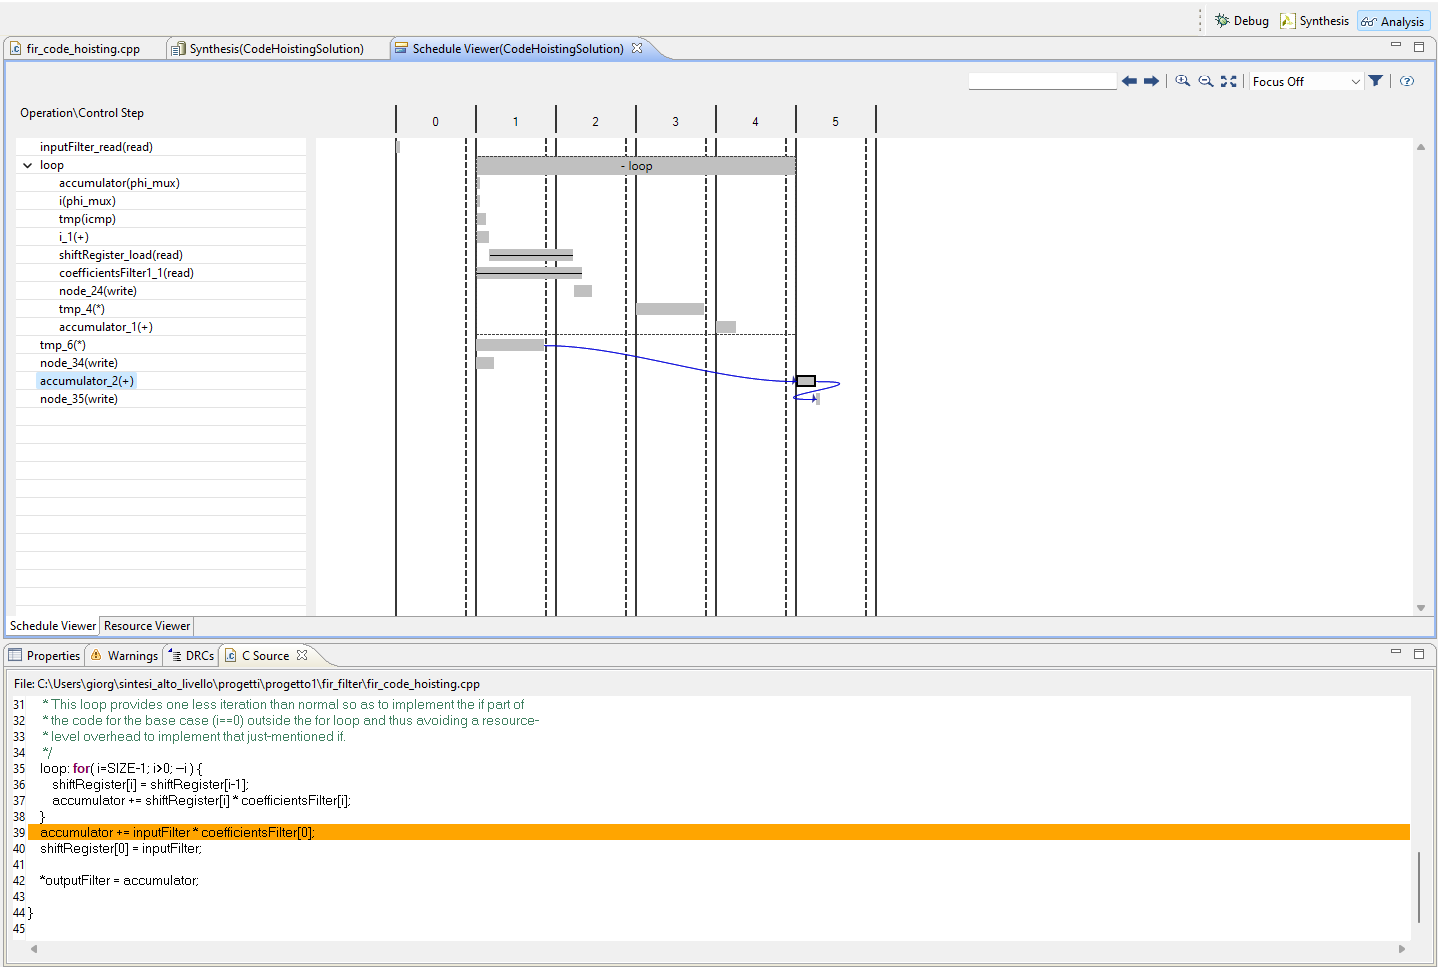
\includegraphics[width=1\textwidth]{solutions/code_hoisting/codehoistinganalysis.png}
    \caption{HLS Code Hoisting Solution Trip Count Analysis}
\end{figure}

In particolare, è opportuno fare un'attenta riflessione riguardo la latenza totale dell'architettura hardware in questione. Il report di sintesi, effettivamente, ha restituito una stima di tale valore pari a 42 dal momento bisogna considera una latenza totale del loop pari a 40, un ciclo di latency ulteriore dovuto alla lettura iniziale dell'input (come avviene per ogni soluzione progettata) e, come ultimo, un altro ciclo finale dovuto alle due operazioni in parallelo effettuate: accumulo associato al coefficiente in posizione 0 e scrittura del dato in uscita. Precedentemente, nella soluzione iniziale non ottimizzata, tale latenza finale non era prevista dal momento che il caso $i==0$ veniva gestito all'interno del loop mediante istruzione condizionale e la scrittura del dato in uscita veniva effettuata in parallelo all'operazione appena citata.

\begin{table}[h]
    \centering
    \begin{tabular}{|l|c|c|c|c|}
        \hline
        \textbf{Name}    & \textbf{BRAM\_18K} & \textbf{DSP48E} & \textbf{FF} & \textbf{LUT} \\ \hline
        DSP              & -                   & -               & -           & -            \\ 
        Expression       & -                   & 4               & 0           & 140          \\ 
        FIFO             & -                   & -               & -           & -            \\ 
        Instance         & -                   & -               & -           & -            \\ 
        Memory           & 0                   & -               & 74          & 8            \\ 
        Multiplexer      & -                   & -               & -           & 92          \\ 
        Register         & -                   & -               & 156         & -            \\ \hline
        \textbf{Total}   & 0                   & 4               & 230         & 240          \\ \hline
        \textbf{Available} & 280               & 220             & 106400      & 53200        \\ \hline
        \textbf{Utilization (\%)} & 0            & 1               & $\sim$0     & $\sim$0      \\ \hline
    \end{tabular}
    \caption{HLS Code Hoisting Solution Utilization Estimates Summary}
    \label{tab:hls-code-hoisting-solution-utilization-estimates-summary}
\end{table}

Si può notare come il report di C/RTL Cosimulation evidenzi un ciclo di latenza in meno rispetto alla soluzione hardware iniziale non ottimizzata. Questo è dovuto al fatto che, come precedentemente citato, il loop presenta un'iterazione in meno tale per cui il numero di cicli di clock, affinché venga processato si abbia un risultato in uscita, è pari a 43 rispetto ai 44 corrispondenti alla soluzione non ottimizzata.

\begin{table}[H]
    \centering
    \begin{tabular}{|c|c|c|c|c|c|c|c|}
        \hline
        \multicolumn{1}{|c|}{RTL} & \multicolumn{1}{|c|}{Status} & \multicolumn{3}{c|}{\textbf{Latency}} & \multicolumn{3}{c|}{\textbf{Interval}} \\
        &  & min & avg & max & min & avg & max \\
        \hline
        VHDL & Pass & 42 & 42 & 43 & 42 & 42 & 43 \\
        \hline
    \end{tabular}
    \caption{HLS Code Hoisting Solution C/RTL Cosimulation Summary }
    \label{tab:hls-code-hoisting-solution-cosimulation-summary}
\end{table}

Inoltre, si può notare come il numero di risorse relative alla soluzione hardware in questione risulta essere pressocché il medesimo tranne per il numero di FF che risulta essere ridotto di circa il 18\%.

\begin{table}[H]
    \centering
    \begin{minipage}[t]{0.45\linewidth}
        \centering
        \begin{tabular}{|l|r|}
            \hline
            \textbf{Resource} & \textbf{VHDL} \\
            \hline
            SLICE & 75 \\
            \hline
            LUT & 270 \\
            \hline
            FF & 131 \\
            \hline
            DSP & 2 \\
            \hline
            BRAM & 0 \\
            \hline
            SRL & 0 \\
            \hline
        \end{tabular}
        \caption{HLS Code Hoisting Solution Export RTL Resource Usage}
        \label{tab:hls-code-hoisting-solution-export-rtl-resoruce-usage}
    \end{minipage}
    \hfill
    \begin{minipage}[t]{0.45\linewidth}
        \centering
        \begin{tabular}{|l|r|}
            \hline
            \textbf{Timing} & \textbf{VHDL} \\
            \hline
            CP required & 10.000 \\
            \hline
            CP achieved post-synthesis & 5.745 \\
            \hline
            CP achieved post-implementation & 6.847 \\
            \hline
        \end{tabular}
        \caption{HLS Code Hoisting Solution Export RTL Final Timing}
        \label{tab:hls-code-hoisting-solution-export-rtl-final-timing}
    \end{minipage}
\end{table}

Pertanto, importando l'IP in Vivado e impostando un clock constraint pari a 10ns è possibile analizzare i seguenti report di risorse, timing, potenza dinamica ed energia per singola operazione.
\lstinputlisting[language=VHDL]{solutions/code_hoisting/clk_constraint.xdc}

\begin{table}[H]
    \centering
    \begin{tabular}{|c|c|c|c|c|c|c|}
        \hline
        \textbf{LUT} & \textbf{LUTRAM} & \textbf{FF} & \textbf{BRAM} & \textbf{DSP} & \textbf{IO} & \textbf{BUFG} \\
        \hline
        270 & 32 & 134 & 0 & 2 & 71 & 1 \\
        \hline
    \end{tabular}
    \caption{Vivado Code Hoisting Solution Utilization Report [\#]}
    \label{tab:vivado-code-hoisting-solution-utilization-reproot}
\end{table}

Dal momento che il WNS è diminuito, si può notare come la maximum clock frequency sia diminuita rispetto alla soluzione non ottimizzata.

\begin{table}[H]
    \centering
    \begin{tabular}{|c|c|c|c|}
        \hline
        \textbf{Cycles} [\#] & \textbf{Clock Constraint} [ns] & \textbf{WNS} [ns] & \textbf{Maximum Clock Frequency} [Mhz] \\
        \hline
        43 & 10 & 3.074 & 144.3834825 \\
        \hline
    \end{tabular}
    \caption{Vivado Code Hoisting Solution Timing Report}
    \label{tab:vivado-code-hoisting-solution-timing-reproot}
\end{table}

Per quanto riguarda la potenza dinamica e l'energia per singola operazione, si evidenzia un aumento rispetto alla soluzione iniziale. Si può ipotizzare che, dal punto di vista della potenza, il tool riesca meglio ad ottimizzare direttamente tutte le operazioni relative ad accumulo e shifting nello stesso ciclo, anziché avere 10 operazioni all'interno del loop e una fuori dal ciclo. 
\begin{table}[H]
    \centering
    \begin{tabular}{|c|c|c|c|c|c|c|}
        \hline
        \textbf{BRAM} & \textbf{Clock Enable} & \textbf{Clocks} & \textbf{DSP} & \textbf{Logic} & \textbf{Set/Reset} [mW] & \textbf{Data} \\
        \hline
        0 & 0.370487687 & 1.756788697 & 0.41467679 & 0.838255044 & 3.35E-03 & 1.381990616 \\
        \hline
    \end{tabular}
    \caption{Vivado Code Hoisting Solution Dynamic Power Report [mW]}
    \label{tab:vivado-code-hoisting-solution-dynamic-power-reproot}
\end{table}

\begin{table}[H]
    \centering
    \begin{minipage}[t]{0.45\linewidth}
        \centering
        \begin{tabular}{|c|}
            \hline
            \textbf{Dynamic Total} \\
            \hline
            4.765546238 \\
            \hline
        \end{tabular}
        \caption{Vivado Code Hoisting Solution Dynamic Power Report [mW]}
        \label{tab:vivado-code-hoisting-solution-dynamic-power-reproot}
    \end{minipage}
    \hfill
    \centering
    \begin{minipage}[t]{0.45\linewidth}
        \centering
        \begin{tabular}{|c|}
            \hline
            \textbf{Energy Single Operation} \\
            \hline
            47.65546238 \\
            \hline
        \end{tabular}
        \caption{Vivado Code Hoisting Solution Energy Single Operation Report [pJ]}
        \label{tab:vivado-code-hoisting-solution-energy-single-operation-reproot}
    \end{minipage}
\end{table}

Pertanto, se da una parte si è ottenuto una piccola diminuzione delle risorse avendo gestito l'overhead di risorse dovuto alle istruzioni condizionali presenti all'interno del loop, dall'altra parte si è ottenuto un aumento di circa il 21\% della potenza dinamica rispetto alla soluzione iniziale non ottimizzata.